\section{Backup und Wiederherstellung des Betriebssystems}

Um die Implementationen und Konfigurationen des Pi's abzusichern, wird eine Backup Lösung eingesetzt. Die Sicherung relevanter Daten soll hierbei einem möglichen Defekt oder Inkompatibilität durch Updates o.ä. entgegenwirken.\\
\\
'FauBackup' und 'gitbac' bieten hierbei eine Lösung mittels externer Programme an. Debian bietet jedoch bereits standardmäßig einige Aufrufe welche zur Anlegung von Backups verwendet werden können. Diese wurden im Folgenden in Ubuntu anhand eines Bash Skripts zur Automatisierung getestet und implementiert.\\

\subsection{dd}
Als erste Ausführung wurde der Aufruf 'dd' verwendet. Hierbei wird der Inhalt der gesamten SD Karte als Image Datei abgespeichert.\\

\subsubsection*{1.}
Übersicht der vorhandenen Dateisysteme mittels des Terminalaufrufs 'df'\\
\begin{figure}[ht]
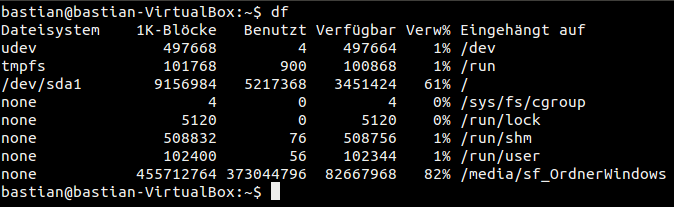
\includegraphics[width=.8\textwidth]{pictures/Bastian/BILD1_df}
\end{figure}

\subsubsection*{2.}
Terminalaufruf für den Backupprozess
\lstset{language=bash,numbers=none,frame=single}
\begin{lstlisting}
sudo dd if=INPUTPARTITION of=OUTPUTFILE
\end{lstlisting}
\begin{tabular}{l c l}
sudo	& -> & Backupprozess benötigt root-Rechte\\
dd	& -> & bit-genaues Kopieren der Dateien\\
if=FILE	& -> & Die Datei oder Partition welche integriert wird\\
of=FILE & -> & Die Output Datei welche angelegt wird\\
\end{tabular}
\newpage %==============================================

\subsubsection*{3.}
Optionale Nutzung von Terminalaufruf 'pv' um den Fortschritt des Backup Prozesses zu sehen Die mögliche Restzeit lässt sich nur durch das Hinterlegen der Größe der Partition anzeigen.
\begin{lstlisting}
sudo dd if=INPUTPARTITION |pv| sudo dd of=OUTPUTFILE
\end{lstlisting}
\begin{figure}[ht]
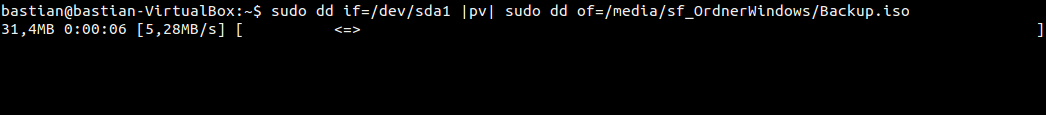
\includegraphics[width=\textwidth]{pictures/Bastian/BILD2_pv}
\end{figure}

\subsubsection*{4.}
Wiederherstellen eines hinterlegten Backups läuft ähnlich wie der ursprüngliche Prozess ab.
\begin{lstlisting}
sudo dd if=OUTPUTFILE |pv| of=INPUTPARTITION
\end{lstlisting}
\begin{figure}[ht]
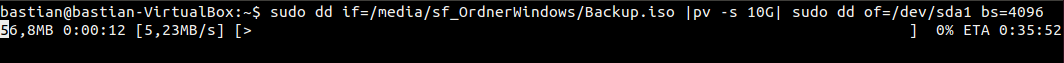
\includegraphics[width=\textwidth]{pictures/Bastian/BILD3_pv}
\end{figure}
\newpage %==============================================

\subsection{rsync}
Da der Vorgang mittels 'dd' als suboptimal angesehen wird, wurde alternativ der Aufruf 'rsync' verwendet. Dieser bietet die Möglichkeit eines inkrementellen Backups wodurch die Dauer des Prozesses erheblich reduziert werden kann. Hierbei werden die Größe und die Änderungszeit der Dateien in Quelle und Ziel miteinander verglichen. Eine Aktualisierung findet demnach nur statt, wenn Unterschiede vorzufinden sind.
\begin{lstlisting}
rsync -aAXv --delete --exclude={"/dev/*","/proc/*","/sys/*","/tmp/*","/run/*","/mnt/*","/media/*","/lost+found"} / /path/to/backup/folder
\end{lstlisting}
\begin{tabular}{l c l}
rsync	&->& Kopieren der Dateien\\
-aAX	&->& Übertragung im Archiv Modus wodurch alle symbolischen Verweise beibehalten werden\\
--delete&->& Dateien die im Ursprungsverzeichnis nicht mehr existieren werden im Zielverzeichnis ebenfalls gelöscht\\
--exclude&->& Dateien werden ausgelassen\\
\end{tabular}
Wiederherstellen des Rsync Backups durch folgenden Befehl:
\begin{lstlisting}
rsync -aAXv /path/to/backup/location/* /mount/point/of/new/install/ --exclude={/dev/*,/proc/*,/sys/*,/tmp/*,/run/*,/mnt/*,/media/*,/lost+found,/home/*}
\end{lstlisting}

\subsection{tar} %===============================================================================
Eine weitere Anwendungsmöglichkeit bietet die 'tar' Archivierung. Vorteil dieses Aufrufs ist, dass durch Angabe von Parametern die Berechtigungen aller zu sichernden Daten ebenfalls beibehalten werden und die Archivierung Speicherplatz spart.\\
Wechsel in das Backupverzeichnis dann:
\begin{lstlisting}
tar -cpzf Backup.tar ORDNER
\end{lstlisting}
\begin{tabular}{l l}
tar	&-> Archivieren von Daten\\
-c	&-> Archiv wird erzeugt (create)\\
-p	&-> Berechtigungen beibehalten (privilige)\\
-z	&-> Zusätzliche Komprimierung mit gzip\\
-f	&-> Archiv in Datei schreiben (finish)\\
\end{tabular}
\newpage %==============================================

\subsection{Automatisierung mittels Bash-Skript} %===============================================
Damit der Nutzer die Aufrufe nicht händisch zu bestimmten Zeiten ausführen muss, wurden zwei Bash-Skripte zur Automatisierung geschrieben. Es gibt ein monatliches Backup mittels (tar) und wöchentliche inkrementelle Backups (rsync) auf die zurückgegangen werden kann.\\
\\
Um das Zeitintervall der Backups einzustellen wird der 'Cron' Dienst verwendet.
Hiermit können Skripte und Programme zu festgelegten Zeiten gestartet werden.
Wenn ein hinterlegter Job täglich zu einer bestimmten Uhrzeit ausgeführt wird muss allerdings auch der Rechner zu dem Zeitpunkt aktiv sein. Ist dies nicht der Fall, startet der Prozess nicht. Um dies zu umgehen wird 'Anacron' verwendet.
Durch ablegen des Skripts in eines der entsprechenden Verzeichnisse wird der Prozess entsprechend ausgeführt.\\
\begin{tabular}{l l}
/etc/cron.hourly/	&- Stündlich ausführen\\
/etc/cron.daily/	&- Täglich ausführen\\
/etc/cron.weekly/	&- Wöchentlich ausführen\\
/etc/cron.monthly/	&- Monatlich ausführen\\
\end{tabular}
\begin{figure}[ht]
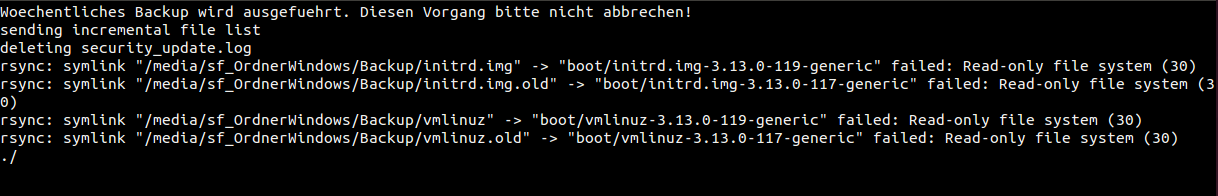
\includegraphics[width=\textwidth]{pictures/Bastian/Woechentliches_Backup}
\end{figure}












